
\documentclass{standalone}
\usepackage[svgnames]{xcolor}
\usepackage{pgfplots}
\pgfplotsset{compat=newest}
\usepackage[sfdefault]{FiraSans}
\usepackage{FiraMono}
\renewcommand*\familydefault{\sfdefault}
\begin{document}
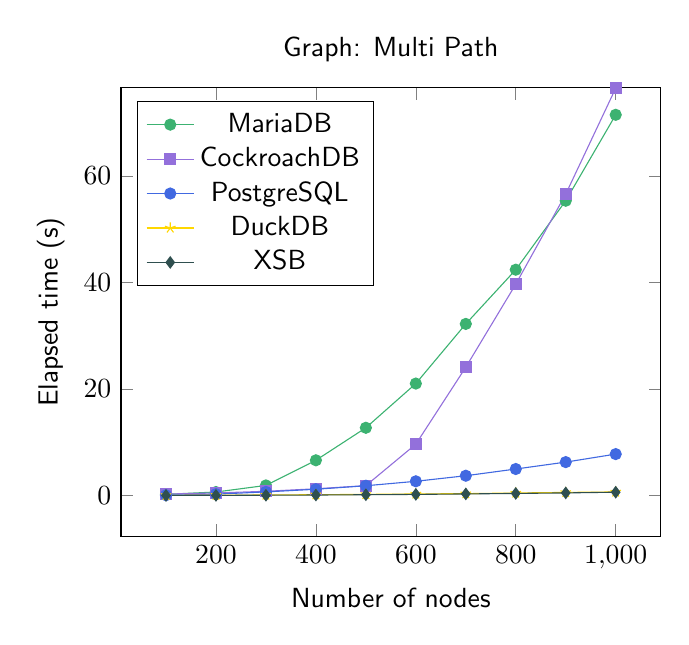
\begin{tikzpicture}
    \begin{axis}[
        title={Graph: Multi Path},
        xlabel={Number of nodes},
        ylabel={Elapsed time (s)},
        legend pos={north west},
        ymax=76.53208919160534
    ]
    \addplot+[MediumSeaGreen, mark options={color=MediumSeaGreen}] coordinates {(100,0.21600307498592883) (200,0.6476330165984109) (300,1.885683475015685) (400,6.605111608188599) (500,12.710034225019626) (600,21.01279040861409) (700,32.21158320840914) (800,42.39028225000948) (900,55.34138327515684) (1000,71.47547184999567)};
\addlegendentry{MariaDB}
\addplot+[MediumPurple, mark options={color=MediumPurple}] coordinates {(100,0.2677182918181643) (200,0.468862416583579) (300,0.7847177419927902) (400,1.2573333833832294) (500,1.8420477084000595) (600,9.629859274998307) (700,24.082580566604157) (800,39.673220183409285) (900,56.57979265039321) (1000,76.47439557478064)};
\addlegendentry{CockroachDB}
\addplot+[RoyalBlue, mark options={color=RoyalBlue}] coordinates {(100,0.050591449998319146) (200,0.24869315839605405) (300,0.6687914500012994) (400,1.1652802829979918) (500,1.8244078915915451) (600,2.6598712333943695) (700,3.705717966798693) (800,4.966204825392924) (900,6.263408558396622) (1000,7.767165766377002)};
\addlegendentry{PostgreSQL}
\addplot+[Gold, mark options={color=Gold}] coordinates {(100,0.019246842002030463) (200,0.04960389179177582) (300,0.08738652499159798) (400,0.14328304962255062) (500,0.20120203340193257) (600,0.2841136080096476) (700,0.34045147520955654) (800,0.465240750007797) (900,0.5728003668133169) (1000,0.660284125211183)};
\addlegendentry{DuckDB}
\addplot+[DarkSlateGray, mark options={color=DarkSlateGray}] coordinates {(100,0.004955005645751952) (200,0.02030463218688964) (300,0.04639101028442384) (400,0.0843867778778076) (500,0.1376051902770996) (600,0.20166959762573242) (700,0.286094045639038) (800,0.3830055713653566) (900,0.4792084217071532) (1000,0.6148792266845702)};
\addlegendentry{XSB}

    \end{axis}
\end{tikzpicture}
\end{document}
